\documentclass[12pt,a4paper]{article}

\usepackage[utf8]{inputenc}
\usepackage[T1]{fontenc}
\usepackage{polski}

\usepackage{amsthm}
\usepackage{amsmath}
\usepackage{amsfonts}
\usepackage{amssymb}
\usepackage{pgfplots}
\usepackage{tikz}
\usepackage{lmodern}	%fancy font
\usepackage{textcomp}

\usepackage{indentfirst}
\usepackage{graphicx}
\usepackage{caption}
\usepackage{subcaption}
\usepackage{siunitx}
\usepackage{here}


\setlength{\textheight}{24cm}
\setlength{\textwidth}{15.92cm}
\setlength{\footskip}{10mm}
\setlength{\oddsidemargin}{0mm}
\setlength{\evensidemargin}{0mm}
\setlength{\topmargin}{0mm}
\setlength{\headsep}{5mm}
\usepackage{tikz}
\usepackage{lmodern}	%fancy font
\usepackage{textcomp}

\usepackage{graphicx}
\usepackage{caption}
\usepackage{subcaption}
\usepackage{siunitx}
\usepackage{here}


\begin{document}

\begin{table}[H]
\centering
\label{my-label}
\begin{tabular}[width=\textwidth, height=0.5]{|c|c|}
\hline									           					&                           \\

\includegraphics[height=3cm]{img/logo}             					& \textbf{Technika cyfrowa} \\ \hline
\textbf{Temat ćwiczenia} 					& \textbf{Numer ćwiczenia}  \\
Przerzutniki i rejestry	& 3                         \\ \hline
\textbf{Wykonawca}       & \textbf{Ocena}            \\
Łukasz Nawojowski          &                           \\ \hline
\end{tabular}
\end{table}

\section{Cel ćwiczenia}
Zapoznanie się z różnymi rodzajami przerzutników i zbudowanie z nich rejestrów SISO, SIPO, PIPO i PISO.

\newpage
\section{Przebieg ćwiczenia}
\subsection{Asynchroniczny przerzutnik RS}
\begin{figure}[H]
\centering
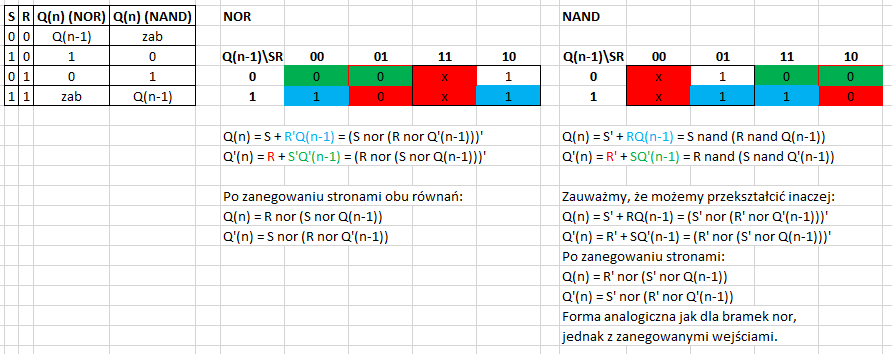
\includegraphics[width=\textwidth]{img/3a_karnaugh}
\end{figure}
\begin{figure}[H]
\centering
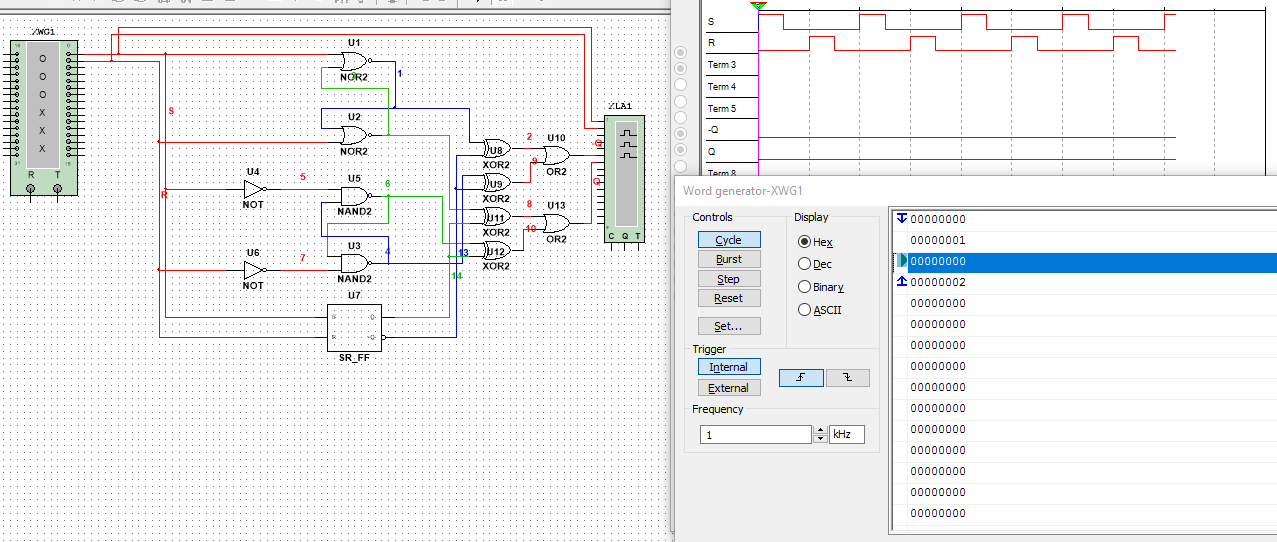
\includegraphics[width=\textwidth]{img/3a}
\end{figure}

Widzimy, że przerzutnik działa zgodnie z przewidywaniami. Przerzutnik oparty o bramki NAND działa tak, jakbyśmy zanegowali wejścia przerzutnika opartego o bramki NOR.

\subsection{Synchroniczny przerzutnik RS}
\begin{figure}[H]
\centering
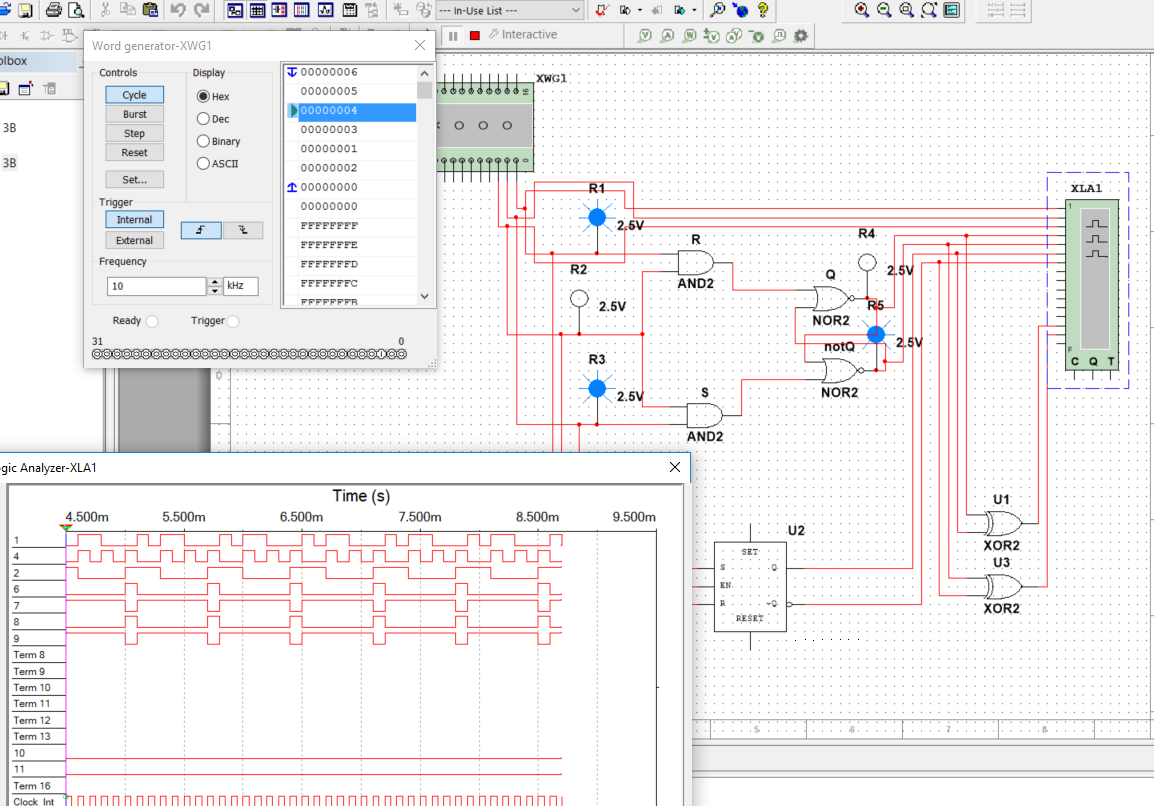
\includegraphics[width=\textwidth]{img/3b}
\end{figure}

\begin{figure}[H]
\centering
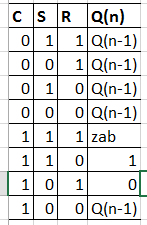
\includegraphics{img/3bTruthTable}
\end{figure}

Synchroniczny przerzutnik RS zmienia stan swoich wyjść tylko, gdy wejście zegara jest w stanie wysokim. Z analizy wyjść układu widać, że zmontowany przerzutnik działa poprawnie. Przerzutniki synchroniczne mogą służyć do konstruowania układów, których działanie jest skoordynowane w czasie, np. procesorów.

\subsection{Synchroniczny przerzutnik JK}
\begin{figure}[H]
\centering
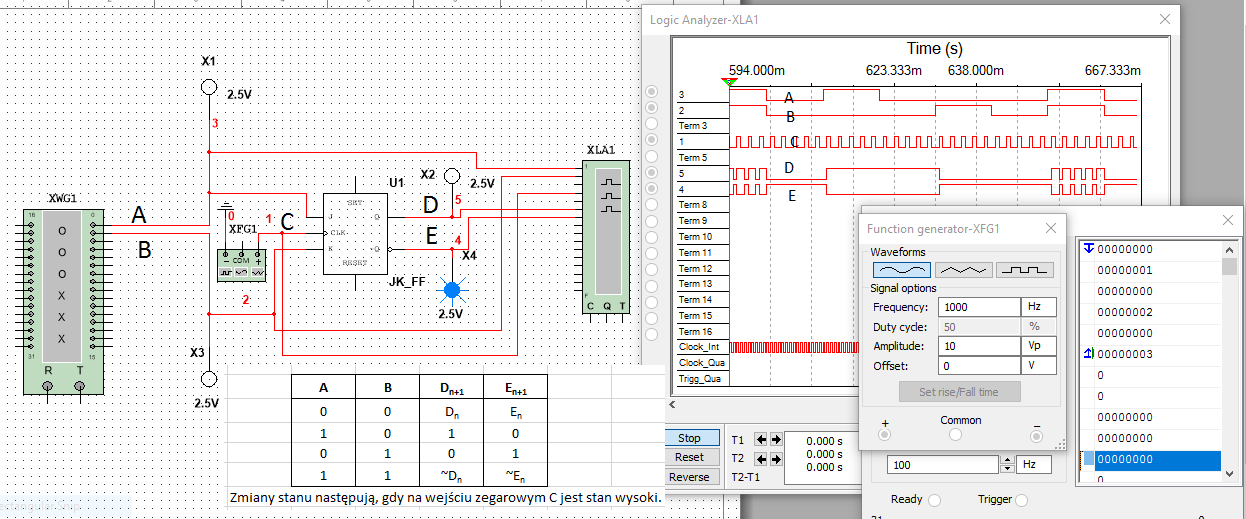
\includegraphics[width=\textwidth]{img/3c_syncJK}
\end{figure}

\begin{figure}[H]
\centering
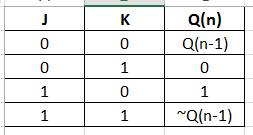
\includegraphics{img/3cTruthTable}
\end{figure}

Przerzutnik JK podobnie do przerzuntika RS ma dwa wejścia: zerujące i jedynkujące. W Multisimie wygenerowano wykres sygnału wyjściowego przerzutnika i porównano z tabelą prawdy, uzyskano zgodność. Przerzutnik reaguje na niski stan syganału zegarowego dzięki zanegowaniu go na wejściu.

Przerzutnik tego typu mógłby służyć na przykład jako konwerter sinusoidalnego sygnału zegarowego na prostokątny.


\subsection{Przerzutnik D na podstawie asynchronicznego przerzutnika RS}
\begin{figure}[H]
\centering
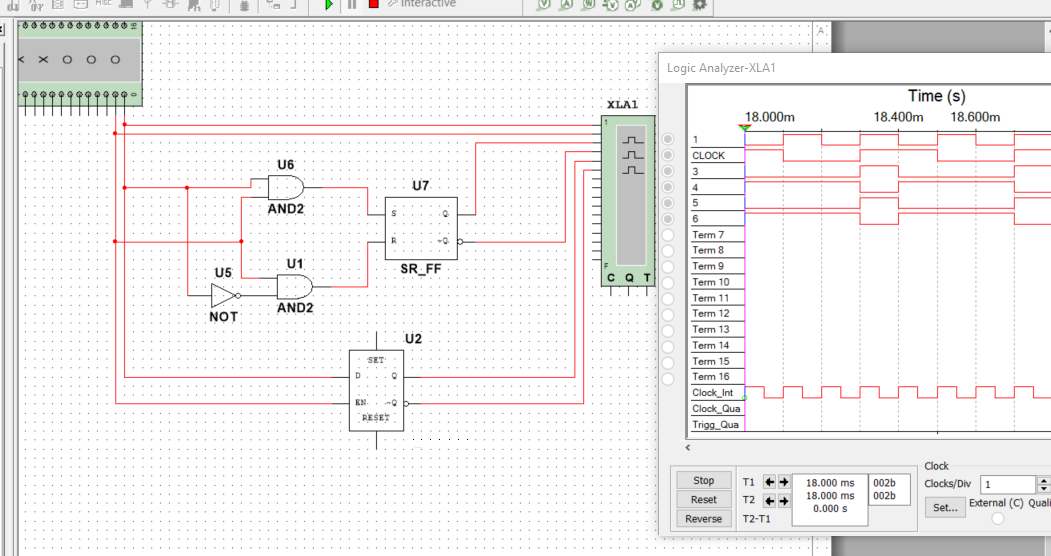
\includegraphics[width=\textwidth]{img/3d}
\end{figure}
\begin{figure}[H]
\centering
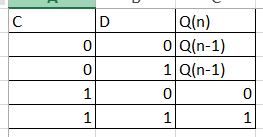
\includegraphics[width=0.6\textwidth]{img/3dTruthTable}
\end{figure}

Nazwa przerzutnika pochodzi z j. angielskiego - od słowa \textit{data} lub \textit{delay}. Jest to układ opóźniający - przepisuje sygnał wejściowy, ale tylko przy odpowiednim sygnale zegara. Jest to zatem także układ synchroniczny.

Przerzutnik D jest przydatny przy budowie rejestrów.

\subsection{Przerzutnik T na podstawie synchronicznego przerzutnika D}
\begin{figure}[H]
\centering
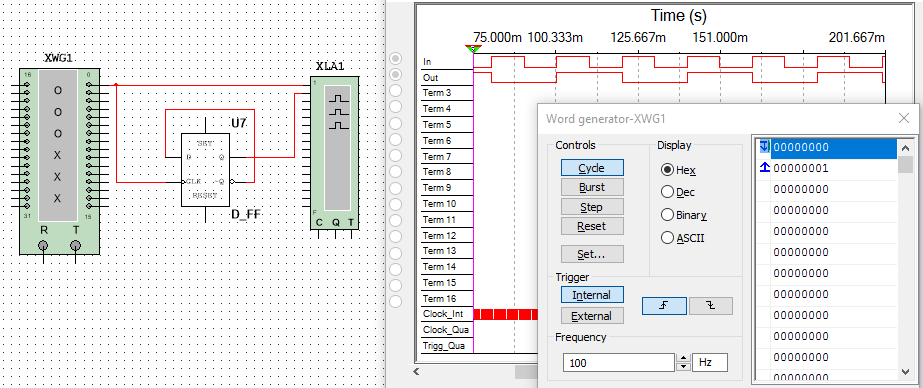
\includegraphics[width=\textwidth]{img/3e}
\end{figure}
\begin{figure}[H]
\centering
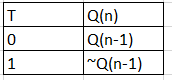
\includegraphics[width=0.2\textwidth]{img/3eTruthTable}
\end{figure}

Okazuje się, że do konstrukcji przerzutnika musimy potraktować wejście zegarowe jako wejście logiczne, co jest ciekawym wykorzystaniem praktycznym konstrukcji.

\newpage
\subsection{Przerzutnik D na podstawie synchronicznego przerzutnika JK}
\begin{figure}[H]
\centering
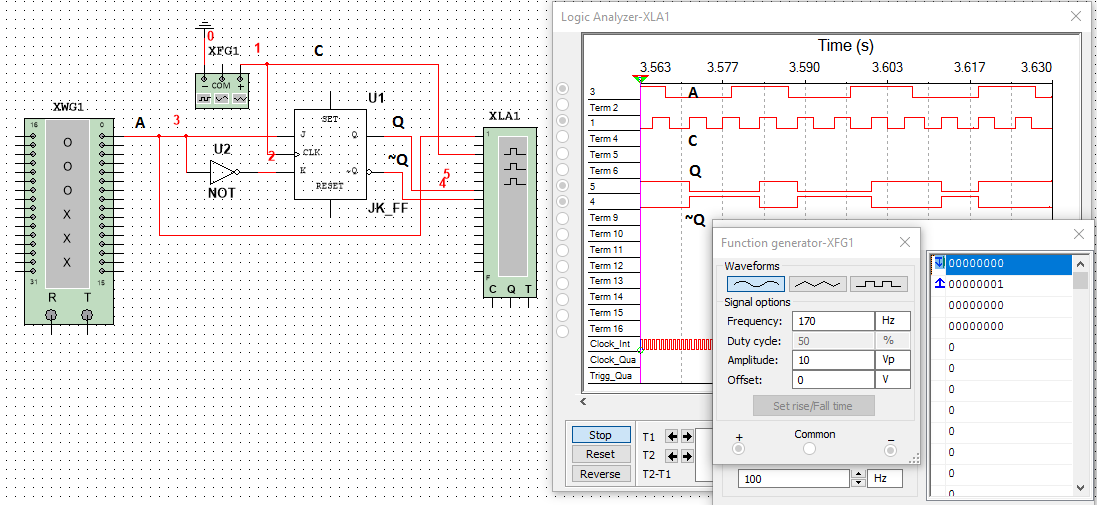
\includegraphics[width=\textwidth]{img/3f}
\end{figure}
\begin{figure}[H]
\centering
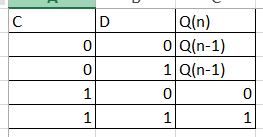
\includegraphics[width=0.3\textwidth]{img/3dTruthTable}
\end{figure}

Widzimy, że możemy symulować funkcje układu z jednym wejściem logicznym przy pomocy układu o dwóch wejściach logicznych.

\newpage
\subsection{Przerzutnik T na podstawie synchronicznego przerzutnika JK}
\begin{figure}[H]
\centering
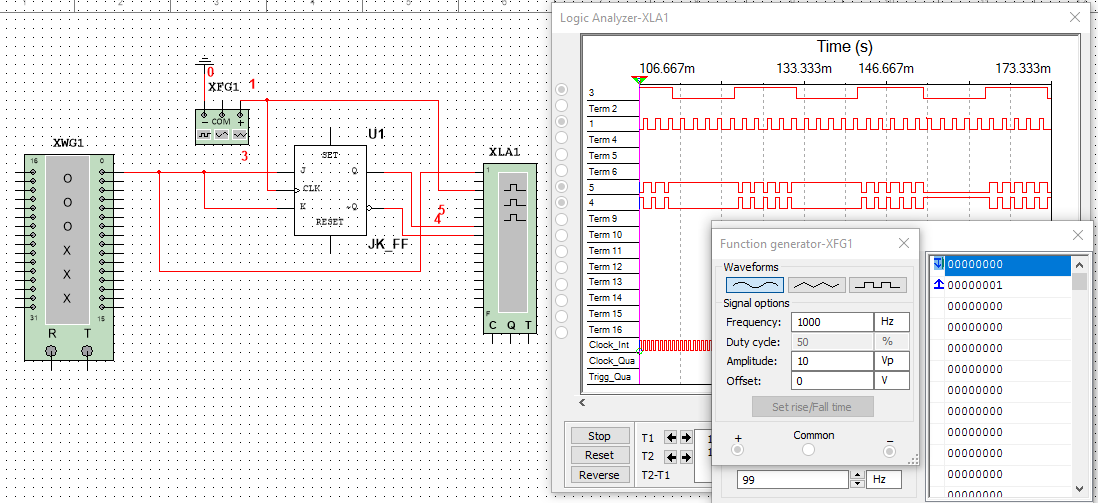
\includegraphics[width=\textwidth]{img/3g}
\end{figure}

Powyższy układ ilustruje budowę przerzutnika T za pomocą przerzutnika JK. Przerzutnik JK okazuje się być  niezwykle uniwersalnym układem.

\newpage
\subsection{Rejestry na podstawie synchronicznych przerzutników D}
\subsubsection{Rejestr PIPO}
\begin{figure}[H]
\centering
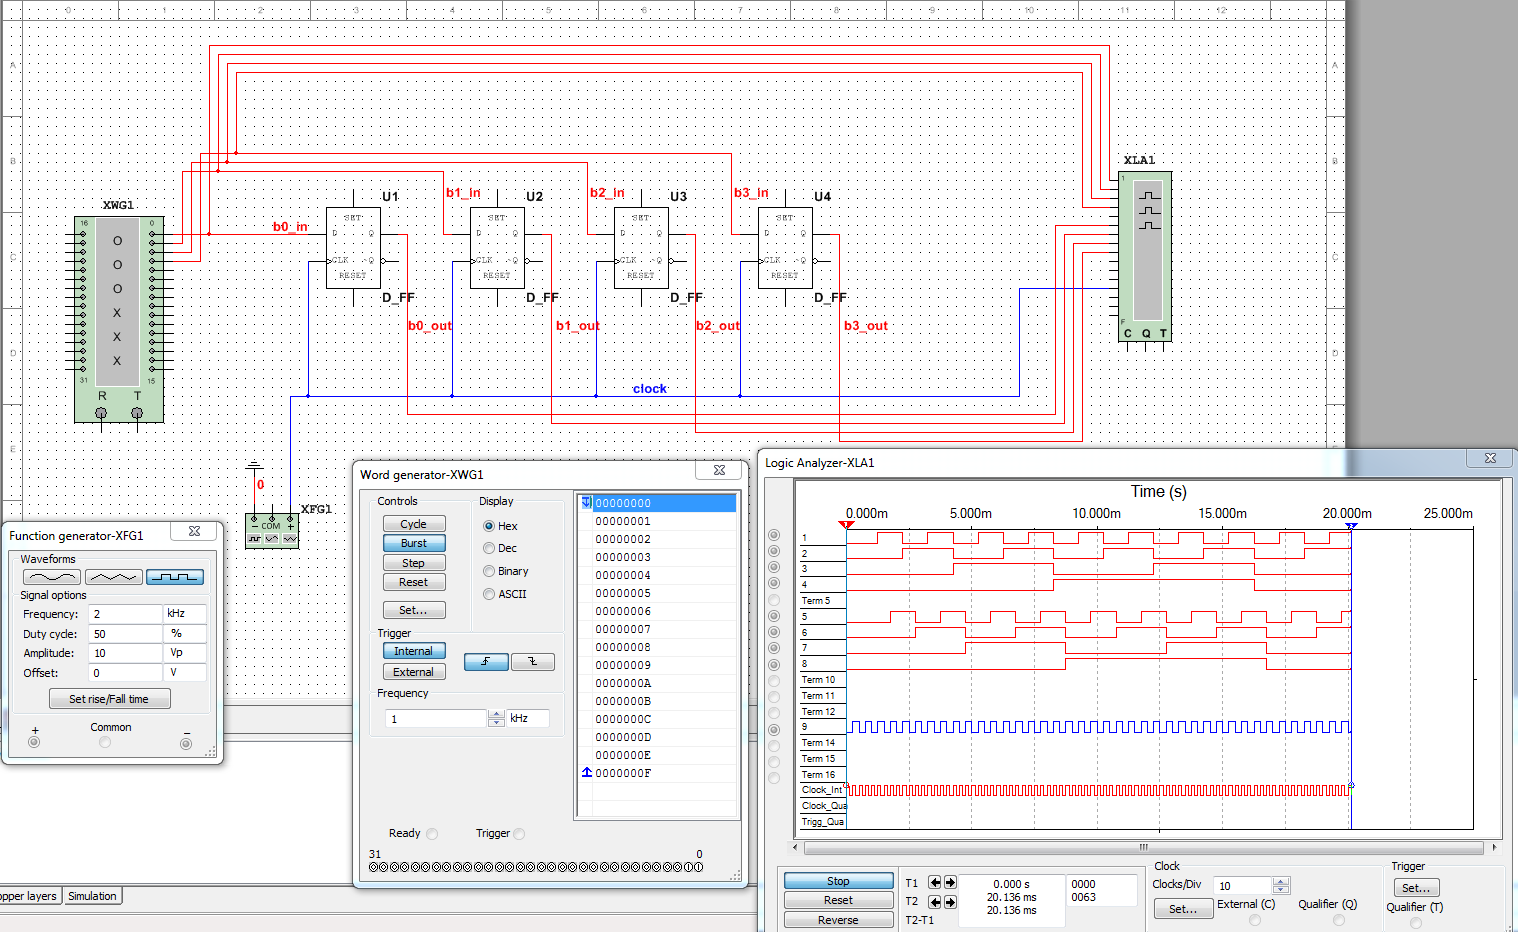
\includegraphics[width=\textwidth]{img/3hPIPO}
\end{figure}
\textbf{PIPO - Parallel-In Parallel-Out} - równoległe wejścia i równoległe wyjścia, czyli wejście i wyjście rejestru jest "szyną" 4 bitową - w każdym z przerzutników sygnał zmieniany jest tylko, gdy dany jest odpowiedni sygnał z zegara.

\subsubsection{Rejestr SIPO}
\begin{figure}[H]
\centering
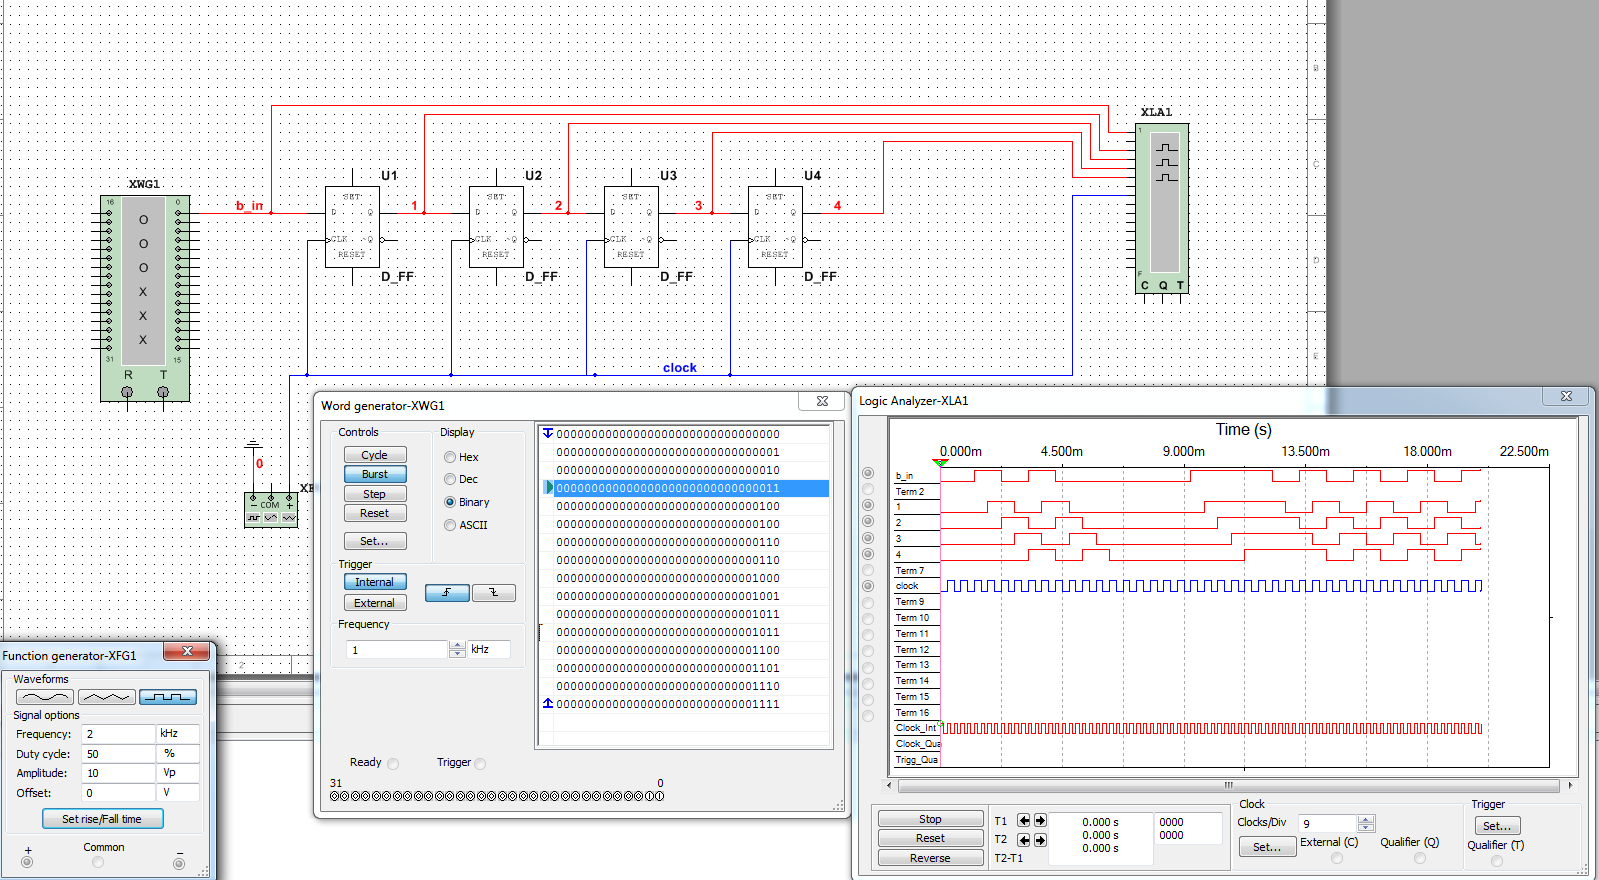
\includegraphics[width=\textwidth]{img/3hSIPO}
\end{figure}

\textbf{SIPO - Serial-In Parallel-Out} - szeregowe wejście, równoległe wyjście - na pojedynczym wejściu podajemy ciąg bitów, a na wyjściu dostajemy 4 równoległe bity. Wejście każdego kolejnego przerzutnika D podłączamy do wyjścia poprzedniego, wejście pierwszego z nich podłączamy do źródła danych. Wyjście każdego z przerzutników to kolejne bity wyjścia rejestru. Z każdym kolejnym cyklem zegara bity przesuwają się w prawo.
Bit najbardziej po prawej jest tracony, najbardziej po lewej jest odczytywany z wejścia szeregowego.

\subsubsection{Rejestr PISO}
\begin{figure}[H]
\centering
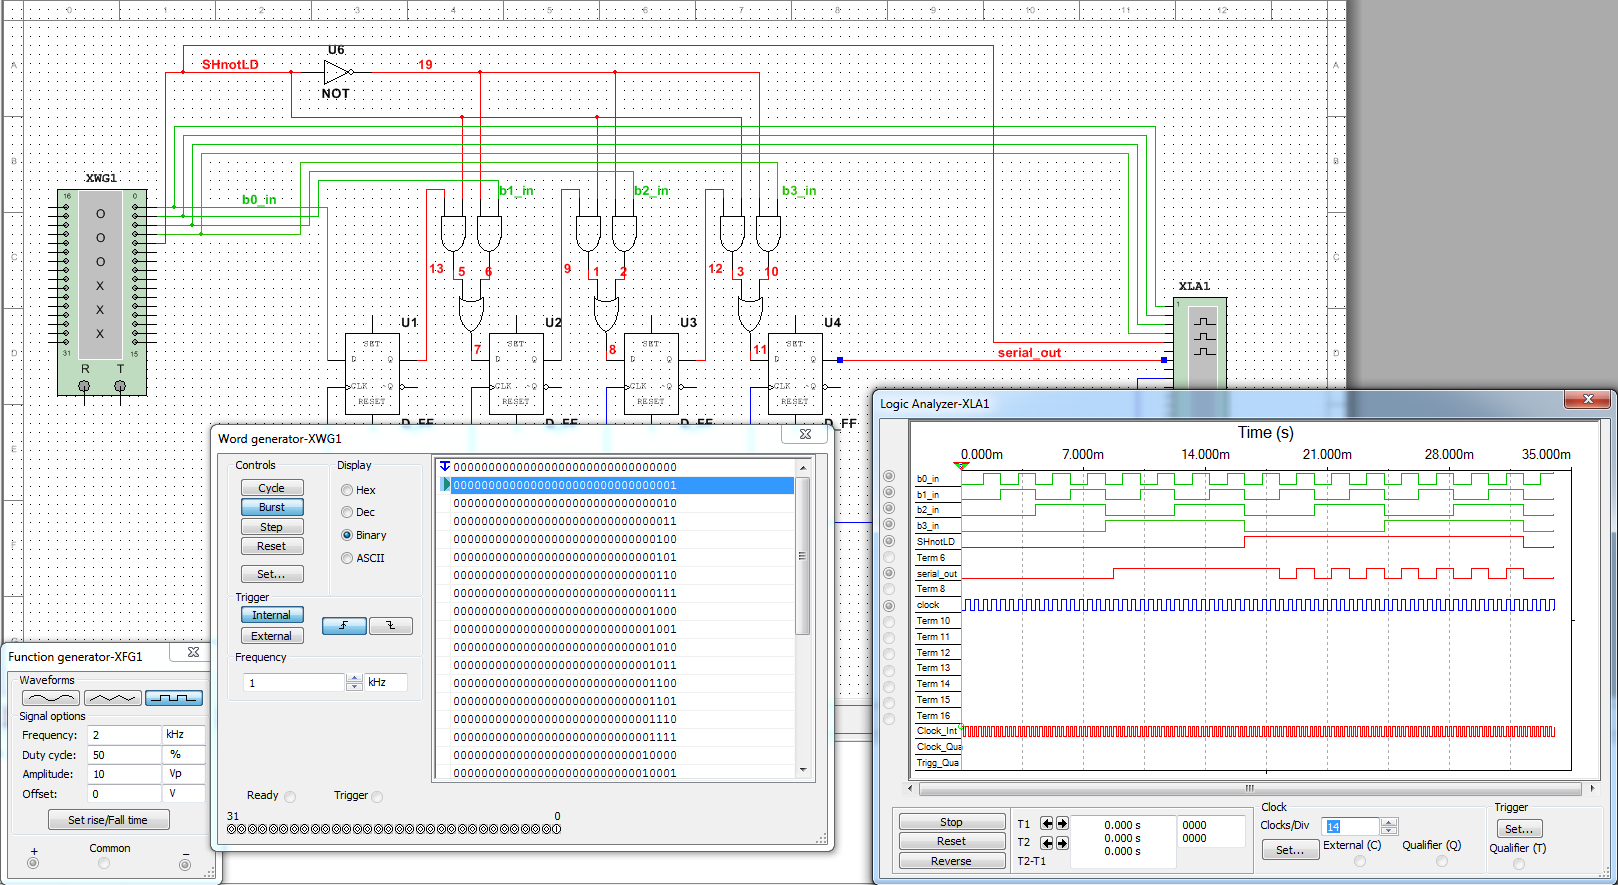
\includegraphics[width=\textwidth]{img/3hPISO}
\end{figure}

\textbf{PISO - Parallel-In Serial-Out} - na wejściu podajemy wiele sygnałów (równolegle), zaś na wyjściu otrzymujemy sygnał szeregowy. Potrzebna jest  możliwość wybrania - czy przesuwamy liczbę w rejestrze w prawo, czy też wczytujemy nową liczbę do rejestru wieloma wejściami. Osiąga się to następującą metodą:


Korzystamy z elementu o nazwie multiplekser - na wejściu dostaje on sterujący sygnał jednobitowy i dwa sygnały jednobitowe (źródła), między którymi będzie przełączał. W zależności od wartości sygnału sterującego, na wyjściu multipleksera pojawia się albo sygnał z jednego źródła, albo z drugiego. W tym wypadku jednym ze źródeł jest wyjście poprzedniego rejestru (bo chcemy móc przesuwać bity w rejestrze), a drugim jest wejście danych (czyli miejsce, skąd chcemy wpisać dane do rejestru). Do każdego wejścia równoległego oprócz pierwszego dodajemy taki multiplekser. Sygnałem sterującym jest SHnotLD - jeżeli sygnał sterujący jest wysoki to wykonujemy SHift - przesunięcie, a jeżeli jest niski, to wykonujemy LoaD - załadowanie nowej liczby do rejestru.

\subsubsection{Rejestr SISO}
\begin{figure}[H]
\centering
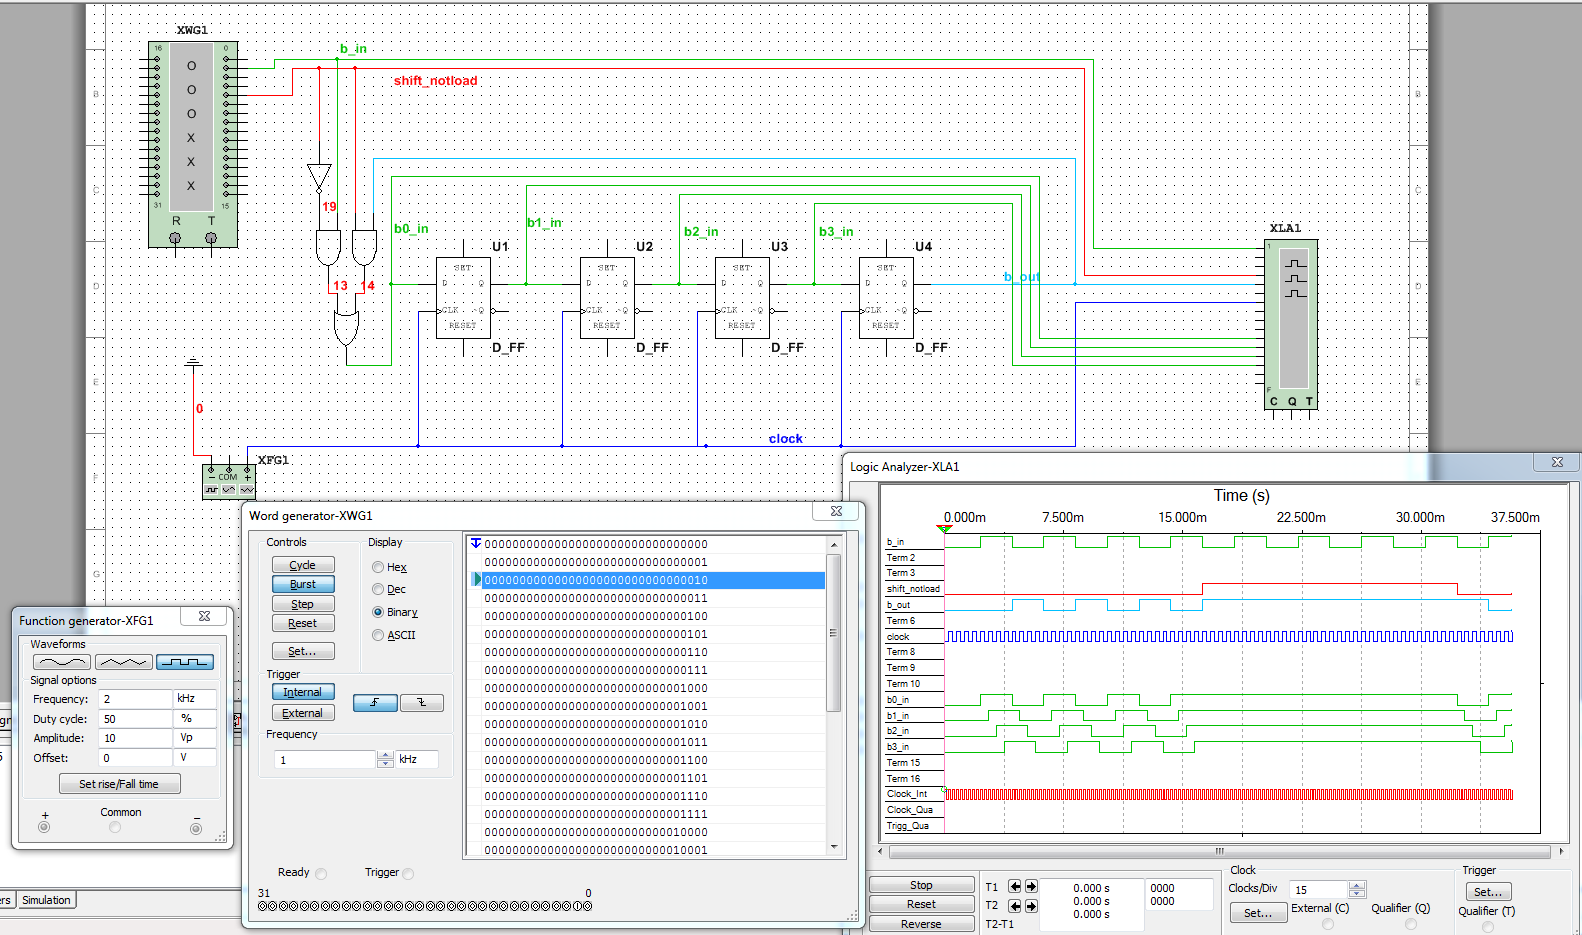
\includegraphics[width=\textwidth]{img/3hSISO}
\end{figure}

\textbf{SISO - Serial-In Serial-Out} - ten rejestr szeregowo dostaje dane i szeregowo ma je zwrócić. Ponieważ na wejściu dostajemy cały czas jakiś sygnał, to chcemy zapobiec utracie tego, co w rejestrze jest. Dlatego tutaj też stosujemy multiplekser korzystający z sygnału SHnotLD, tym razem jednak używamy go, żeby "zapętlić" wyjście szeregowe z wejściem. Wtedy sygnałem SHnotLD, wybieramy czy przesuwamy dalej dane w prawo gubiąc stare (dla sygnału 1 SHnotLD), czy też zapętlamy wyjście z wejściem, czyli efektywnie to co było w rejestrze, będzie się w nim zapętlać.


\section{Wnioski}
Dowiedziałem się, jak działają różne typy przerzutników, jak stosować tabele Karnaugh do rozwiązywania "rekursywnych" funkcji logicznych oraz jak przerzutniki mogą posłużyć ku wyjściu na kolejny poziom abstrakcji - do zbudowania rejestrów, skąd już tylko niewielki krok do asemblera i języków wysokiego poziomu.

\end{document}
